\documentclass[a4paper,11pt]{article}
\usepackage{a4wide}
\usepackage[english]{babel}
\usepackage{europs}
\usepackage{graphicx}

\setlength{\parskip}{1ex}
\setlength{\parindent}{0mm}

\begin{document}
\title{Snow White and the Seven Dwarfs}
\author{Jacob Grimm\\j.grimm@tue.nl \and Wilhelm Grimm\\w.grimm@tue.nl}
\date{}
\maketitle

\begin{figure}[!ht]
\begin{center}
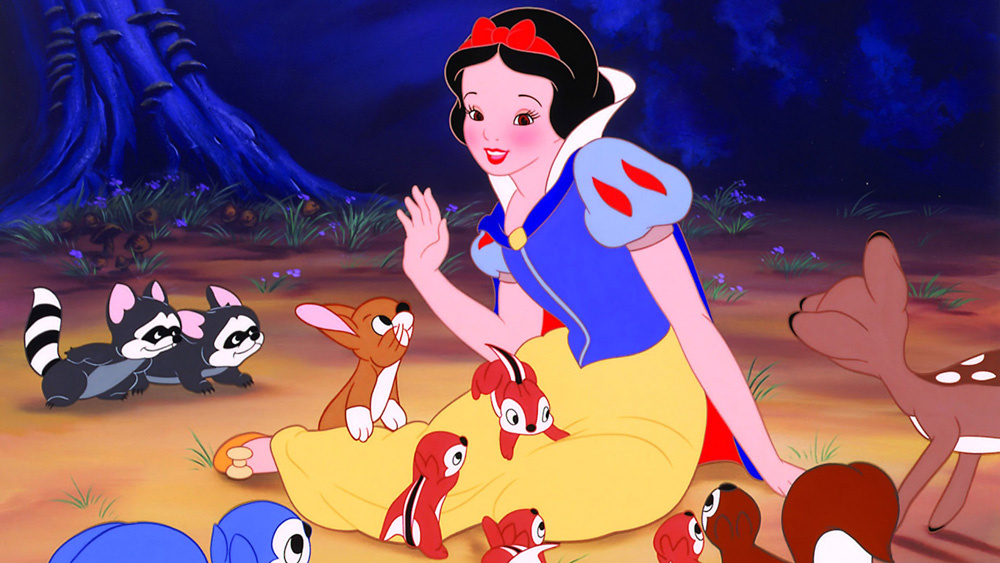
\includegraphics[bb=0 0 250 327,height=5cm]{snowwhite.jpg}
\caption{picture of snowwhite}
\label{fig:snowwhite}
\end{center}
\end{figure}

\begin{abstract}
\noindent
Snow White was a princess who lived long, long ago. Her mother died
and her father remarried. Her new stepmother wants to kill her because
Snow White is more beautiful than she is. Then Snow White runs away and
hides in a small cottage that belongs to seven dwarfs. The stepmother
finds her and kills her. A noble prince comes and kisses her back to
life and marries her. The stepmother goes to the marriage where she gets killed.
\end{abstract}


\tableofcontents
\section{Introduction}

Once upon a time in the middle of winter, when the flakes of
snow were falling like feathers from the sky, a queen sat at
a window sewing, and the frame of the window was made of black
ebony.  And whilst she was sewing and looking out of the window
at the snow, she pricked her finger with the needle, and three
drops of blood fell upon the snow.  And the red looked pretty
upon the white snow, and she thought to herself, would that I had
a child as white as snow, with lips as red as blood, and hair as black as the
wood of the window-frame.

Soon after that she had a little daughter, who was as white as
snow, her lips were as red as blood, and her hair was as black as ebony,
and she was therefore called little snow-white.  And when the
child was born, the queen died.

\section{The evil stepmother}

After a year had passed the king took to himself another wife.
She was a beautiful woman, but proud and haughty, and she could
not bear that anyone else should surpass her in beauty.  She
had a wonderful looking-glass, and when she stood in front of it
and looked at herself in it, and said,
\begin{quote}
          looking-glass, looking-glass, on the wall,\\
          who in this land is the fairest of all.
\end{quote}

The looking-glass answered,
          thou, o queen, art the fairest of all.

Then she was satisfied, for she knew that the looking-glass spoke
the truth.

But snow-white was growing up, and grew more and more beautiful,
and when she was seven years old she was as beautiful as the day,
and more beautiful than the queen herself.  And once when the
queen asked her looking-glass,
          looking-glass, looking-glass, on the wall,
          who in this land is the fairest of all.

It answered,
          thou art fairer than all who are here, lady queen.
          But more beautiful still is snow-white, as I ween.

Then the queen was shocked, and turned yellow and green with
envy.  From that hour, whenever she looked at snow-white, her
heart heaved in her breast, she hated the girl so much.
And envy and pride grew higher and higher in her heart like a
weed, so that she had no peace day or night.  She called a
huntsman, and said, take the child away into the forest.  I will
no longer have her in my sight.  Kill her, and bring me back her
lung and liver as a token.  The huntsman obeyed, and took her away
but when he had drawn his knife, and was about to pierce
snow-white's innocent heart, she began to weep, and said, ah dear
huntsman, leave me my life.  I will run away into the wild forest,
and never come home again.

And as she was so beautiful the huntsman had pity on her and
said, run away, then, you poor child.  The wild beasts will soon
have devoured you, thought he, and yet it seemed as if a stone had
been rolled from his heart since it was no longer needful for
him to kill her.  And as a young bear just then came running by
he stabbed it, and cut out its lung and liver and took them to the
queen as proof that the child was dead.  The cook had to salt them,
and the wicked queen ate them, and thought she had eaten the lung
and liver of snow-white.


\section{The great forest}

But now the poor child was all alone in the great forest, and so
terrified that she looked at all the leaves on the trees, and did
not know what to do.  Then she began to run, and ran over sharp
stones and through thorns, and the wild beasts ran past her, but
did her no harm.

She ran as long as her feet would go until it was almost evening,
then she saw a little cottage and went into it to rest herself.
Everything in the cottage was small, but neater and cleaner than
can be told.  There was a table on which was a white cover, and
seven little plates, and on each plate a little spoon, moreover,
there were seven little knives and forks, and seven little mugs.
Against the wall stood seven little beds side by side, and
covered with snow-white counterpanes.

\section{The seven dwarfs}
\subsection{The cottage}

Little snow-white was so hungry and thirsty that she ate some
vegetables and bread from each plate and drank a drop of wine
out of each mug, for she did not wish to take all from one only.
Then, as she was so tired, she laid herself down on one of the
little beds, but none of them suited her, one was too long,
another too short, but at last she found that the seventh one was
right, and so she remained in it, said a prayer and went to
sleep.

\subsection{The dwarfs}

When it was quite dark the owners of the cottage came back.
They were seven dwarfs who dug and delved in the mountains for
ore.  They lit their seven candles, and as it was now light within
the cottage they saw that someone had been there, for everything
was not in the same order in which they had left it.


\begin{enumerate}
\item The first said, who has been sitting on my chair.
\item The second, who has been eating off my plate.
\item The third, who has been taking some of my bread.
\item The fourth, who has been eating my vegetables.
\item The fifth, who has been using my fork.
\item The sixth, who has been cutting with my knife.
\item The seventh, who has been drinking out of my mug.
\end{enumerate}

Then the first looked round and saw that there was a little
hollow on his bed, and he said, who has been getting into my
bed.  The others came up and each called out, somebody has been
lying in my bed too.  But the seventh when he looked at his bed
saw little snow-white, who was lying asleep therein.  And he
called the others, who came running up, and they cried out with
astonishment, and brought their seven little candles and let the
light fall on little snow-white.  Oh, heavens, oh, heavens, cried
they, what a lovely child.  And they were so glad that they did
not wake her up, but let her sleep on in the bed.  And the
seventh dwarf slept with his companions, one hour with each, and
so passed the night.


\subsection{The encounter}

When it was morning little snow-white awoke, and was frightened
when she saw the seven dwarfs.  But they were friendly and asked
her what her name was.  My name is snow-white, she answered.
How have you come to our house, said the dwarfs.  Then she told
them that her step-mother had wished to have her killed, but
that the huntsman had spared her life, and that she had run for
the whole day, until at last she had found their dwelling.

The dwarfs said, if you will take care of our house, cook, make
the beds, wash, sew and knit, and if you will keep everything neat
and clean you can stay with us and you shall want for nothing.
Yes, said snow-white, with all my heart.  And she stayed with
them.  She kept the house in order for them.  In the mornings
they went to the mountains and looked for copper and gold, in the
evenings they came back, and then their supper had to be ready.
The girl was alone the whole day, so the good dwarfs warned her
and said, beware of your step-mother, she will soon know that you
are here, be sure to let no one come in.


\section{The murder of Snow White}
\subsection{First attempt}

But the queen, believing that she had eaten snow-white's lung and
liver, could not but think that she was again the first and most
beautiful of all, and she went to her looking-glass and said,
looking-glass, looking-glass, on the wall,
          who in this land is the fairest of all.

And the glass answered,
          oh, queen, thou art fairest of all I see,
          but over the hills, where the seven dwarfs dwell,
          snow-white is still alive and well,
          and none is so fair as she.

Then she was astounded, for she knew that the looking-glass
never spoke falsely, and she knew that the huntsman had betrayed
her, and that little snow-white was still alive.

And so she thought and thought again how she might kill her,
for so long as she was not the fairest in the whole land, envy let
her have no rest.  And when she had at last thought of something
to do, she painted her face, and dressed herself like an old
pedlar-woman, and no one could have known her.  In this disguise
she went over the seven mountains to the seven dwarfs, and
knocked at the door and cried, pretty things to sell, very cheap,
very cheap.  Little snow-white looked out of the window and called
out, good-day my good woman, what have you to sell.  Good things,
pretty things, she answered, stay-laces of all colors, and she
pulled out one which was woven of bright-colored silk.  This lace
is very cheap: it only costs \EURofc 5, which is a bargain, because on the
Internet you won't find it below \$10. Just check e-bay! I may let
the worthy old woman in, thought snow-white, and she unbolted the
door and bought the pretty laces.  Child, said the old woman,
what a fright you look, come, I will lace you properly for once.
Snow-white had no suspicion, but stood before her, and let herself
be laced with the new laces.  But the old woman laced so quickly
and so tightly that snow-white lost her breath and fell down as
if dead.  Now I am the most beautiful, said the queen to herself,
and ran away.

Not long afterwards, in the evening, the seven dwarfs came home,
but how shocked they were when they saw their dear little snow-white
lying on the ground, and that she neither stirred nor
moved, and seemed to be dead.  They lifted her up, and, as they
saw that she was laced too tightly, they cut the laces, then she
began to breathe a little, and after a while came to life again.
When the dwarfs heard what had happened they said, the old
pedlar-woman was no one
else than the wicked queen, take care and let no one come in
when we are not with you.


\subsection{Second attempt}

But the wicked woman when she had reached home went in front
of the glass and asked,
          looking-glass, looking-glass, on the wall,
          who in this land is the fairest of all.

And it answered as before,
          oh, queen, thou art fairest of all I see,
          but over the hills, where the seven dwarfs dwell,
          snow-white is still alive and well,
          and none is so fair as she.

When she heard that, all her blood rushed to her heart with fear,
for she saw plainly that little snow-white was again alive.
But now, she said, I will think of something that shall really
put an end to you.  And by the help of witchcraft, which she
understood, she made a poisonous comb.  Then she disguised
herself and took the shape of another old woman.  So she went
over the seven mountains to the seven dwarfs, knocked at the
door, and cried, good things to sell, cheap, cheap.  Little
snow-white looked out and said, go away, I cannot let anyone come
in.  I suppose you can look, said the old woman, and pulled the
poisonous comb out and held it up.  It pleased the girl so well
that she let herself be beguiled, and opened the door.  When they
had made a bargain the old woman said, now I will comb you
properly for once.  Poor little snow-white had no suspicion, and
let the old woman do as she pleased, but hardly had she put the
comb in her hair than the poison in it took effect, and the girl
fell down senseless.  You paragon of beauty, said the wicked
woman, you are done for now, and she went away.

But fortunately it was almost evening, when the seven dwarfs
came home.  When they saw snow-white lying as if dead upon the
ground they at once suspected the step-mother, and they looked
and found the poisoned comb.  Scarcely had they taken it out when
snow-white came to herself, and told them what had happened.
Then they warned her once more to be upon her guard and to open
the door to no one.


\subsection{Third attempt}

The queen, at home, went in front of the glass and said,
          looking-glass, looking-glass, on the wall,
          who in this land is the fairest of all.

Then it answered as before,
          oh, queen, thou art fairest of all I see,
          but over the hills, where the seven dwarfs dwell,
          snow-white is still alive and well,
          and none is so fair as she.

When she heard the glass speak thus she trembled and shook
with rage.  Snow-white shall die, she cried, even if it costs me
my life.

Thereupon she went into a quite secret, lonely room, where no
one ever came, and there she made a very poisonous apple.
Outside it looked pretty, white with a red cheek, so that
everyone who saw it longed for it, but whoever ate a piece of it
must surely die.

When the apple was ready she painted her face, and dressed herself
up as a farmer's wife, and so she went over the seven
mountains to the seven dwarfs.  She knocked at the door.  Snow-white
put her head out of the window and said, I cannot let
anyone in, the seven dwarfs have forbidden me.  It is all the
same to me, answered the woman, I shall soon get rid of my apples.
There, I will give you one.

No, said snow-white, I dare not take anything.  Are you afraid
of poison, said the old woman, look, I will cut the apple in two
pieces, you eat the red cheek, and I will eat the white.  The
apple was so cunningly made that only the red cheek was
poisoned.  Snow-white longed for the fine apple, and when she saw
that the woman ate part of it she could resist no longer, and
stretched out
her hand and took the poisonous half.  But hardly had she a bit
of it in her mouth than she fell down dead.  Then the queen
looked at her with a dreadful look, and laughed aloud and said,
white as snow, red as blood, black as ebony-wood, this time the
dwarfs cannot wake you up again.

And when she asked of the looking-glass at home,
          looking-glass, looking-glass, on the wall,
          who in this land is the fairest of all.

And it answered at last,
          oh, queen, in this land thou art fairest of all.
Then her envious heart had rest, so far as an envious heart can
have rest.


\section{The funeral}

The dwarfs, when they came home in the evening, found snow-white
lying upon the ground, she breathed no longer and was dead.
They lifted her up, looked to see whether they could find
anything poisonous, unlaced her, combed her hair, washed her
with water and wine, but it was all of no use, the poor child was
dead, and remained dead.  They laid her upon a bier, and all
seven of them sat round it and wept for her, and wept three days
long.

Then they were going to bury her, but she still looked as if she
were living, and still had her pretty red cheeks.  They said,
we could not bury her in the dark ground, and they had a
transparent coffin of glass made, so that she could be seen from
all sides, and they laid her in it, and wrote her name upon it
in golden letters, and that she was a king's daughter.  Then they
put the coffin out upon the mountain, and one of them always
stayed by it and watched it.  And birds came too, and wept for
snow-white, first an owl, then a raven, and last a dove.

And now snow-white lay a long, long time in the coffin, and she
did not change, but looked as if she were asleep, for she was as
white as snow, as red as blood, and her hair was as black as
ebony.


\section{The prince}

It happened, however, that a king's son came into the forest, and
went to the dwarfs, house to spend the night.  He saw the coffin
on the mountain, and the beautiful snow-white within it, and read
what was written upon it in golden letters.  Then he said to the
dwarfs, let me have the coffin, I will give you whatever you want
for it.  But the dwarfs answered, we will not part with it for all
the gold in the world.  Then he said, let me have it as a gift, for
I cannot live without seeing snow-white.  I will honor and prize
her as my dearest possession.  As he spoke in this way the good
dwarfs took pity upon him, and gave him the coffin.

And now the king's son had it carried away by his servants on
their shoulders.  And it happened that they stumbled over a
tree-stump, and with the shock the poisonous piece of apple
which snow-white had bitten off came out of her throat.  And
before long she opened her eyes, lifted up the lid of the coffin,
sat up, and was
once more alive.  Oh, heavens, where am I, she cried.  The king's
son, full of joy, said, you are with me.  And told her what had
happened, and said, I love you more than everything in the
world, come with me to my father's palace, you shall be my wife.


\section{The marriage}

And snow-white was willing, and went with him, and their wedding
was held with great show and splendor.  But snow-white's
wicked step-mother was also bidden to the feast.  When she had
arrayed herself in beautiful clothes she went before the
looking-glass, and said,
          looking-glass, looking-glass, on the wall,
          who in this land is the fairest of all.

The glass answered,
          oh, queen, of all here the fairest art thou,
          but the young queen is fairer by far as I trow.

Then the wicked woman uttered a curse, and was so wretched,
so utterly wretched that she knew not what to do.  At first she
would not go to the wedding at all, but she had no peace, and
had to go to see the young queen.  And when she went in she
recognized snow-white, and she stood still with rage and fear,
and could not stir.  But iron slippers had already been put upon
the fire, and they were brought in with tongs, and set before
her.  Then she was forced to put on the red-hot shoes, and dance
until she dropped down dead. Snow-white, the prince, the prince's
horse and most of the seven dwarfs lived happily ever after.

\begin{center}
                         \Huge The End
\end{center}
\end{document}